\documentclass[10pt,a4paper]{article}
\usepackage[utf8]{inputenc}
\usepackage{amsmath}
\usepackage{amsfonts}
\usepackage{amssymb}
\usepackage{graphicx}
\author{José Jácome}
\title{Resolución de EDP y EDO mediante Matlab}
\begin{document}
\setlength{\unitlength}{1 cm} %Especificar unidad de trabajo
\thispagestyle{empty}
\begin{picture}(18,4)
\put(-3,0){
\includegraphics[scale=0.5]{ESPE.png}}
\put(9.5,0){
\includegraphics[scale=0.25]{Mecatronica.png}}
\end{picture}
\\
\\
\begin{center}
\textbf{{\Huge UNIVERSIDAD DE LAS FUERZAS ARMADAS}\\[0.5cm]
{\LARGE ESPE EXTENSIÓN LATACUNGA}}\\[1.25cm]
{\Large MATEMÁTICA SUPERIOR}\\[2.3cm]
{\LARGE \textbf{EDO y EDP con MATLAB}}\\[3.5cm]
{\large Jácome José}\\[2cm]
IV MECATRÓNICA "A"\\[1cm]
Latacunga-Ecuador - \today
\end{center}

\section{Métodos de una resolución de EDO}
\subsection*{Integrales y Derivadas}
Para resolver una ecuacion diferencial ordinaria EDO, podemos utilizar los conceptos que ya conocemos en Matlab. Como demostracion, examinaremos la siguiente ecuacion diferencial:

 \begin{center}
 $\frac{d^2y}{{dx}^2}=7x^3-\frac{1}{x^4}$
 \end{center}
Integrando en ambos extremos con respecto a la variable independiente

\begin{center}
$\int \frac{d^2y}{{dx}^2}dx=\int (7x^3-\frac{1}{x^4})dx$
\end{center}

Obtenemos 
\begin{center}
 $\frac{dy}{dx}=\frac{7x^4}{4}-\frac{1}{x^3}+C_1$
\end{center}

Integramos nuevamente
\begin{center}
$\int \frac{dy}{dx}dx=\int (\frac{7x^4}{4}-\frac{1}{x^3}+C_1)dx$
\end{center}

Obtenemos la ecuacion General:
$y=\frac{7}{20}x^6-\frac{1}{x^2}+C_1x+C_2$
\\
Realizando lo mismo en Matlab, podemos ingresar los siguientes comandos:






Como se observa, hemos llegado a la misma respuesta. Ahora bien, dado que Matlab no agrega las constantes de integracion, nosotros mismos debemos agregarlas, simplemente creandolas como variables aleatorias con {\bf syms}, y sumandolas en la operacion de integracion
\\
Para el ejemplo anterior, dado que debiamos integrar dos veces, habia que sumar la primera costante de integracion en la primera operacion, y la segunda constante de integracion en la segunda operacion

\subsection*{Metodos de separacio de variables}
Sea la siquiente ecuacion diferencial:

\begin{center}
$\frac{dy}{dx}=\frac{xy+3x-y-3}{xy-2x+4y-8}$
\end{center}

Resolverla utilizando integracion: En Matlab, utilizaremos los comandos {\bf simple}, para simplificar (o factorizar) la expresion:

Ahora en nuestra cabeza (o en nuestro cuaderno) reescribir la ecuacion para que nos quede en la forma deseada:

\begin{center}
$\frac{y-2}{y+3}dy=\frac{x-1}{x+4}dx$
\end{center}

Para resolverla por este metodo, y obtener el valor de la constante de integracion, debemos de igualar a cero:

\begin{center}
$\frac{y-2}{y+3}dy-\frac{x-1}{x+4}dx=0$
\end{center}

Escribiendo en Matlab, tenemos:




Por lo que nuestra solucion general es:

\begin{center}
$C=y-5 \ln(y+3)-x+5 \ln(x+4)$
\end{center}

Ahora, necesitamos una solucion particular para $y_{(0)}=1$; por lo que se entiende que $x=0$ y $y=1$; entonces, simplemente le damos valores fijos a las variables aleatorias {\bf x} e {\bf y}, y utilizamos {\bf eval} para calcular nuevamente C:













\section*{Comando dsolve}
Este comando ayuda a facilitar la resolucion de EDO's, pero hay que definir la ecuacion como una cadena de texto
\\
Ahora resolvamos nuevamente el primer ejercicio (Ingresando la ecuacion diferencial en su forma diferencial):


Como puede apreciarse, escribimos la expresion en terminos de t, no de x. Esto se debe a que en el area de investigacion, la mayoria de ecuaciones diferenciales, son en razon del tiempo, por lo que Matlab maneja que toda esta en funcion de t.
\\
Entonces, simplemente, sustituimos x por t en la expresion, y a la respuesta, la sustituimos en viceversa. Note tambien que es importante la notacion de la derivada de y. Por lo cual se puede guiar en la siguiente tabla:

\begin{center}
\begin{tabular}{|c|c| } \hline
 $Escritura$ & $Equivalencia$ \\ \hline
Dy & $\frac{dy}{dt}$ \\ \hline

D2y & $\frac{d^2y}{{dt}^2}$  \\ \hline

D3y & $\frac{d^32y}{{dt}^3}$  \\ \hline

Dny & $\frac{d^ny}{{dt}^n}$\\ \hline

\end{tabular}
\end{center}

Ahora resolveremos un ejercicio ya hecho en el metodod de separacion de variables














Lamentablemente, dado que Matlab busca siempre la respuesta mas exacta, e sposible que algun resultado nos sea expresado en una funcion llamada Lambert $W^1$, la cual, sale por completo de nuestro conocimiento matematico (e innecesario), por fortuna, dicha funcion es una sencilla igualdad:

\begin{center}
$f(z)=W.f(z).e^{W.f(z)}$
\end{center}

Es decir, cuando el elemento multiplicador de la funcion es igual al exponente de $e$ entonces, equivale a unicamente la expresion $f(z)$. Al obtener esta respuesta, hay que realizar un simple truco, repitiendo el proceso, ponga mucha atencion (vamos a escribir en una forma derivativa):










Con el comando {\bf solve}($funcion,'variable'$) hemos despejado la respuesta de la ecuacion diferencial en relacion a $C_1$. Con ello obtenemos una respuesta compacta. Simplemente hacemos caso omiso a todas las (t) en la expresion.
\\
De esto:
\begin{center}
$C_1=-y(t)-5*\ln (\frac{x(t)+4}{y(t)+3})+x(t)$
\end{center}

Llegamos a esto:
\begin{center}
$C_1=-y-5*\ln (\frac{x+4}{y+3})+x$
\end{center}

Ahora expandimos el logaritmo:
\begin{center}
$C_1=-y-5(\ln(x+4)-\ln(y+3))+x$
\end{center}

Realizamos la multiplicacion:
\begin{center}
$C_1=-y-5\ln(x+4)+5\ln(y+3)+x$
\end{center}
  
Ordenamos y finalmente:
\begin{center}
$C_1=-y-5\ln(x+4)+x+5\ln(y+3)$
\end{center}
 
Observe que es la misma respuesta obtenida por integrales, exceptuando que toda la expresion esta multiplicada por un factor de $(1)$. Esto se debe a que dependiendo de la naturaleza de la funcion, posee suspropias restricciones en rango y dominio, por lo que por simetria, la curva $C_1$ es simetrica equivalente a $-C_1$; es decir es la misma traza, con signo diferente
\\
Por elli, el software no puede sustituir las buenas practicas de ejercicios manuales, aunque nos aporta gran ayuda
\\
{\bf No se preocupe, si su respuesta hecha a mano, es de signo contrario a la aportadad por Matlab. !Su respuesta es correcta!, solo que Matlab encontro la respuesta de la traza reflejada}

\section*{Soluciones Particulares con el comando dsolve}

Al comando {\bf dsolve} tambien se le puede agregar condiciones iniciales:

\begin{center}
$dsolve('ecuacion diferencial','condicion inicial')$
\end{center}

Como ejemplo resolvamos la ecuacion diferencial con  condiciones iniciales:

\begin{center}
$(y^3-x^3)dx-(xy^2)dy=0$
\\
con $y(1)=2$
\end{center}

Para que sea facil su ingreso en la linea de comandos, hacemos un cambio de variable x por t:

\begin{center}
$$(y^3-t^3)dt-(ty^2)dy=0$$
\end{center}

Ahora llevamos a la forma diferencial:

\begin{center}
$\frac{dy}{dt}=\frac{y^3-t^3}{ty^2}$
\end{center}

Luego ingresamos en Matlab









El sistema nos devuelve una respuesta en terminos de las variables dependientes, es decir {\bf y}, lo que se interpreta como:

\begin{center}
$y=t{(-3\ln(t)+8)}^{\frac{1}{3}}$
\end{center}

Realizamos el cambio de variable:

\begin{center}
$y=x{(-3\ln(x)+8)}^{\frac{1}{3}}$
\end{center}

Y asi tenemos la solucion particular de la ecuacion. Pero si nos conviene la respuesta expresada en C (es decir el valor unemrico constante en la expresion) debemos trabajar la respuesta a mano:

\begin{center}
$\frac{y}{x}={(-3\ln(x)+8)}^{\frac{1}{3}}$
\\
$\frac{y^3}{x^3}=-3\ln(x)+8$
\end{center}

Llegamos a la respuesta clasica:

\begin{center}
$\frac{y^3}{x^3}+3\ln(x)=8$
\end{center}
\begin{center}
\section{Resolución de Ecuaciones Diferenciales Parciales con Matlab}
\end{center}
\subsection{Comando pdepe} 
El comando \textit{pdepe} se utiliza para resolver 	Ecuaciones Diferenciales Parciales con condiciones iniciales para ecuaciones de tipo parabólico y elíptico\\
Esta permite resolver EDP o sistemas de EDPs de una variable especial x y una variable temporal t. La forma normal de las EDPs, 
\begin{verbatim}
u = pdepe(m,@pdefun,@icfun, @bcfun,x,t)
\end{verbatim}
\subsection{Forma General de las EDP para llevar a Matlab} 
La forma normal que se pueden resolver es de la forma:\\
$c (x,t,u, \dfrac{\partial u}{\partial x}) \dfrac{\partial u}{\partial x} = \dfrac{1}{x^n} \dfrac{\partial}{\partial x} [x^m f(x,t,u,\dfrac{\partial u}{\partial x})] + s(x,t,u, \dfrac{\partial u}{\partial x})$\\
El Coeficiente c que multiplica la derivada con respecto a $t$ es una matriz diagonal que se especifica como vector. La variable especial para 	reescalarse es tener: $0 < x < 1$.\\
El Parámetro m esta asociado a la geometría del problema: m = 0,1,2 corresponde a x como la coordenada radial en coordenadas cartesianas, cilíndricas o esféricas respectivamente. \\
Los terminos $f,s$ se llaman flujo y fuente respectivamente.
\subsection{Condiciones de Frontera}
La condición de frontera en los extremos $x \in [0,1]$ se especifican en la forma:\\
$p(x,t,u) + q(x,t) f(x,t,u,\dfrac{\partial u}{\partial x})$\\
donde $x= a,b$. Es necesario especificar loas componentes de $p = (pl, pr)$ y de $q = (ql,qr)$ como funciones de t y de los valores de u en los extremos $(ul,ur)$ en el caso de p. Note que las condiciones de frontera se especifican mediante el flujo de la derivada parcial $\dfrac{\partial u}{\partial x}$
\subsection{Condiciones Iniciales}
Se especifican en la forma de una función de x\\
$u = icfun(x)$
\subsection{Llamada principal para resolver una EDP}
\begin{verbatim}
u = pdepe(m,@pdefun,@icfun, @bcfun,x,t)
\end{verbatim}
Sean $nx = length(x)$ , $nt = lenght(t)$ las longitudes de las mallas $x$ y $t$ respectivamente, $np$ es el numero de ecuaciones diferenciales, entonces:
\begin{verbatim}
a = x(1) < x(2) < ... <x(end) = b
0 = t(1) < t(2) < ... < t(end)
\end{verbatim}
La solución $u$ es un arreglo multidimensional de tamaño $nt * nx * np$ ; con $nx \geq 3$, por ejemplo $u(j,k,i)$ es la solución aproximada de la componente $i$en el punto $(t(j),x(k))$.
Nótese que los índices $j,k$ corresponden al orden de las variables $(t,x)$.\\
Las funciones en el argumento de pdepe siguen la sintaxis:
\subsection{Flujo} 
\begin{verbatim}
[c,f,s] = pdefun(x,t,u,dudx)
\end{verbatim}
donde $x, t$ son escalares, $u, dudx$ son vectores de dimensión np. La función regresa
vectores c,f,s de de dimensión np correspondientes a la matriz diagonal $c(x,t,u,\dfrac{\partial u}{\partial x} / )$,flujo $f(x,t,u ,\dfrac{\partial u}{\partial x} )$ y fuente $s(x,t,u , \dfrac{\partial u}{\partial x} )$. Por cada entrada del vector c nulo, la ecuación correspondiente es de tipo elíptica pero debe haber al menos una ecuación parabólica.

\subsection{Condiciones de frontera} 
\begin{verbatim}
[pl,ql,pr,qr] = bcfun(xl,ul,xr,ur,t)
\end{verbatim}
donde $pl, ql$ son vectores columna de dimensión np correspondientes a la función $p(a,t,u)$ y a la matriz diagonal $q(a,t,u,\dfrac{\partial u}{\partial x})$. Note que sólo p puede depender de u. Análogamente $pr, qr$ son vectores columna de dimensión
np correspondientes a la función $p(a,t,u)$ y a la matriz diagonal $q(b,t,u ,\dfrac{\partial u}{\partial x})$
\subsection{Condición inicial}
\begin{verbatim}
u = icfun(x)
\end{verbatim}
donde x es un escalar, u es un vector de dimensión np. 
\subsection{Evaluación de la solución en puntos específicos de x} 
\begin{verbatim}
ui = u(:,:,i)
\end{verbatim}
aproxima la i-ésmima componente de la solución en la malla tempo-espacial (t,x).\\
Para evaluar la solución y su derivada en puntos de la malla  $xout$ distintos de la malla x se usa el comando.
\begin{verbatim}
[uout,duoutdx] = pdeval(m,x,ui,xout)
\end{verbatim}
la salida son vectores $uout,duoutdx$ contienen las aproximaciones en la malla $xcout$.\\
Observe que se evalúa la derivada y no el flujo. 
\begin{verbatim}
Manejo de discontinuidades
\end{verbatim} 
Se permiten discontinuidades de cos en x siempre que se incluyan en la malla x, pero el
flujo deberá ser continuo. Es conveniente usar una malla más fina cerca de los puntos de
discontinuidad, pero para m =2 (coordenadas esféricas) esto no es necesario. \\
\subsection{Codigo de Matlab}
\begin{verbatim}
%Resolucion de una EDP por Matlab
function pdex1
% 20 puntos de malla especial, 5 temporal
m = 0;
x = linspace(0,1,20);
t = linspace(0,2,5);
%Llamada a la rutina principal
sol = pdepe(m,@pdex1pde,@pdex1ic,@pdex1bc,x,t);
%Primera componente
u=sol(:,:,1);
%Grafico de superficie
figure;
surf(x,t,u);
title('Solución numérica con 20 puntos de malla.');
xlabel('Distancia x');
ylabel('Tiempo t');
figure;
surf(x,t,exp(-t)'*sin(pi*x));
title('Solución exacta con 20 puntos de malla. ');
xlabel('Distance x');
ylabel('Time t');
figure;
plot(x,u(end,:), 'o',x,exp(-t(end))*sin(pi*x));
title('Soluciones en t = 2. ');
legend('Numerica, 20 puntos de malla', 'Analitica',0);
xlabel('Distancia x'); ylabel('u(x,2)');
% Especificacion de la EDP
function [c,f,s] = pdex1pde(x,t,u,DuDx)
c = pi^2;
f = DuDx;
s = 0;
% Especificación de la condición inicial
function u0 = pdex1ic(x)
u0 = sin(pi*x);
% Especificación de condiciones de frontera
function [pl,ql,pr,qr] = pdex1bc(xl,ul,xr,ur,t)
pl = ul;
ql = 0;
pr = pi * exp(-t);
qr = 1; 

\end{verbatim}
\subsection{Capturas de Pantalla}
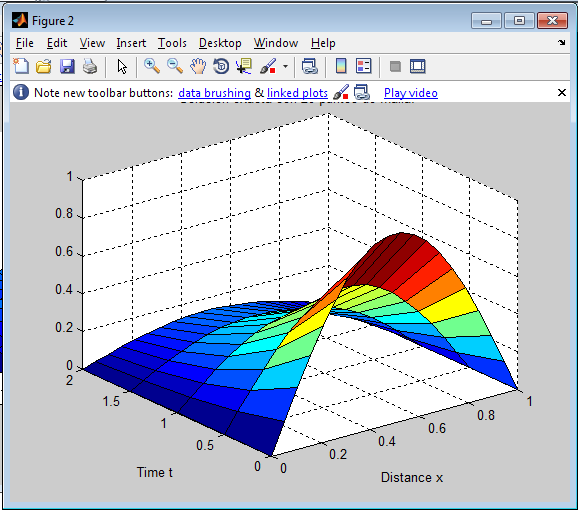
\includegraphics[scale=0.5]{Grafica1.png}\\
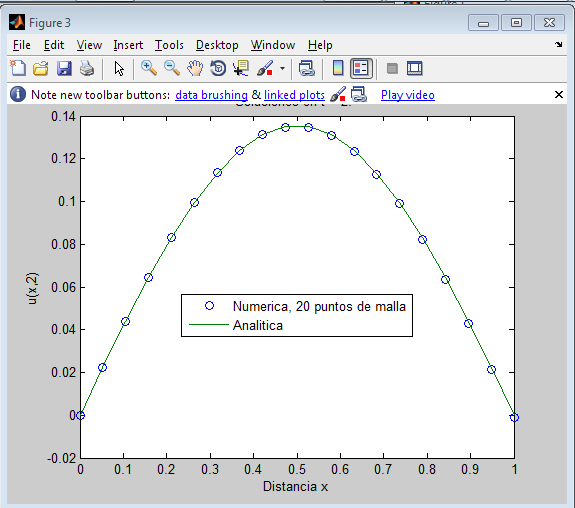
\includegraphics[scale=0.5]{Grafica2.png}
\end{document}